\documentclass[a2,portrait]{a0poster}

\usepackage{multicol} % This is so we can have multiple columns of text side-by-side
\columnsep=60pt % This is the amount of white space between the columns in the poster
\columnseprule=3pt % This is the thickness of the black line between the columns in the poster

\usepackage[svgnames]{xcolor} % Specify colors by their 'svgnames', for a full list of available color names see here: http://www.latex-community.org/forum/viewtopic.php?f=37&t=24668

\usepackage{times} % Use the times font
\usepackage{graphicx} % Required for including images
\usepackage{float}
\graphicspath{{images/}} % Location of the graphics files

\usepackage{booktabs} % Top and bottom rules for table
\usepackage[font=small,labelfont=bf]{caption} % Required for specifying captions to tables and figures

\usepackage[margin=.5in]{geometry}


\begin{document}

%----------------------------------------------------------------------------------------
%	POSTER HEADER 
%----------------------------------------------------------------------------------------

\begin{center}
\begin{minipage}{0.75\textwidth}
\centering
\huge \color{NavyBlue} \textbf{Efficient and low noise toroidal propeller design} \color{Black}\\ % Title
\large \textbf{Louis Pender}\\[0.5cm] % Author(s)
\large Cambridge University Engineering Department\\ % University/department
\end{minipage}
\end{center}

%----------------------------------------------------------------------------------------

\vspace{1cm}

\begin{minipage}[t][0pt]{0.97\linewidth}
\begin{multicols}{2} % Begin the two-column layout 


%----------------------------------------------------------------------------------------
%  PURPOSE
%----------------------------------------------------------------------------------------

\color{Navy}
\section*{Purpose}

Developing low noise propulsion systems is crucial for the aviation industry to address growing public concerns over aircraft noise pollution and facilitate the adoption of innovative technologies, particularly in the context of VTOL aircraft operating in urban environments. Toroidal propellers are one such design that can significantly reduce noise levels compared to conventional propellers, fostering a positive public perception of aviation technologies and enabling the widespread adoption of solutions like urban air mobility and drone-based services.
Efficient design is also essential for propulsion systems to ensure optimal performance and viability in various applications as efficiency directly impacts aircraft range, payload capacity, and overall operational costs.

%----------------------------------------------------------------------------------------
%	OBJECTIVES
%----------------------------------------------------------------------------------------

\vfill\null
\columnbreak

\color{Navy} 
\section*{Objectives}

\begin{itemize}
\item To identify features and select geometric parameters for a toroidal propeller important for efficiency and noise reduction
\item To develop computational models for the prediction of the performance of toroidal propellers.
\item To demonstrate an experimental setup to further test and validate the computational models over a range of design points.
\item To present designs for a range of both audible and effective performance.
\end{itemize}

Figure \ref{fig:noise} from a highlight by MIT \cite{MIT_toroidal} shows the audible noise reduction of toroidal propellers compared to conventional propellers.
This highlight also discussed that the toroidal design can achieve thrust comparable to that of a multirotor drone propeller.
I believe further research into toroidal propellers can provide informed design decisions for efficient and low noise propulsion systems.

%----------------------------------------------------------------------------------------

\end{multicols}

\begin{figure}[H]
    \centering
    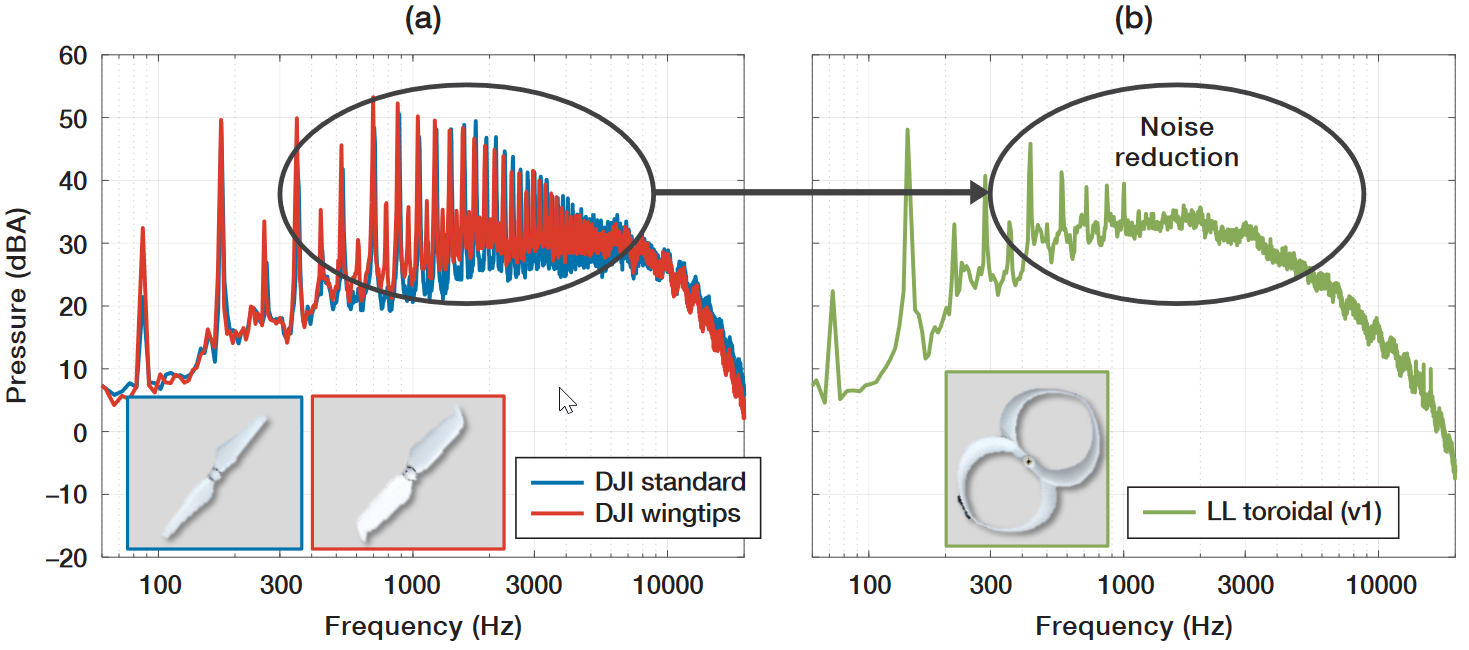
\includegraphics[width=0.8\textwidth]{noise.png}
    \caption{The comparison between conventional propellers used on DJI's quadrotors (a) and the toroidal propeller (b)
    shows the significant reduction of discernible noise achieved by the toroidal propeller. \cite{MIT_toroidal}}
    \label{fig:noise}
\end{figure}


%----------------------------------------------------------------------------------------
%	REFERENCES
%----------------------------------------------------------------------------------------

\color{Black} 

\begin{thebibliography}{9}

    \bibitem{MIT_toroidal}
      MIT Lincoln Laboratory,
      \emph{Innovation Highlight: Toroidal Propeller}.
      2022.
    
\end{thebibliography}

\end{minipage}
\end{document}
